\documentclass[border=6pt]{standalone}
\usepackage{tikz}
\usetikzlibrary{arrows.meta,positioning}
\usepackage[scaled]{helvet}
\renewcommand{\familydefault}{\sfdefault}
\begin{document}
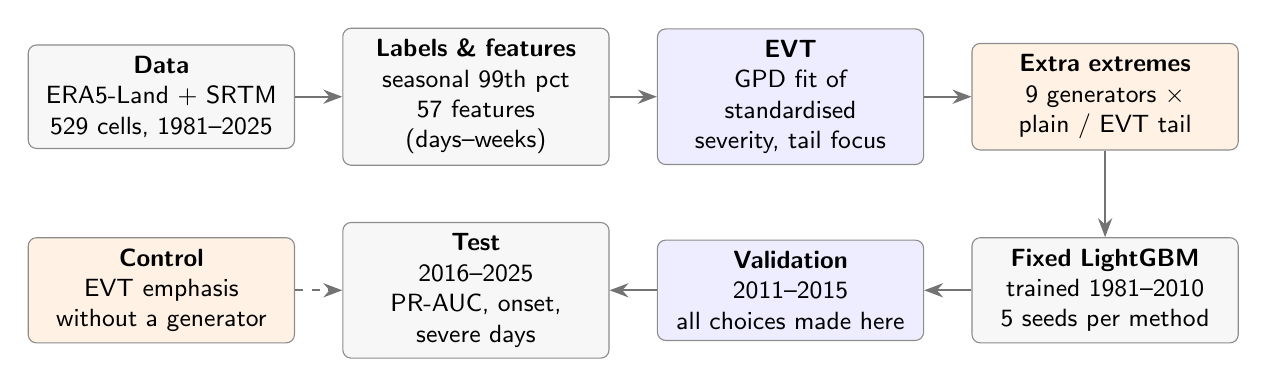
\begin{tikzpicture}[
  box/.style={draw=black!45, rounded corners=3pt, fill=#1, align=center, font=\small,
              minimum height=1.25cm, text width=3.1cm, inner sep=4pt},
  box/.default={black!3},
  arr/.style={-{Stealth[length=2.4mm]}, thick, black!55}]
\node[box] (data) {\textbf{Data}\\ERA5-Land + SRTM\\529 cells, 1981--2025};
\node[box, right=0.6cm of data] (lab) {\textbf{Labels \& features}\\seasonal 99th pct\\57 features (days--weeks)};
\node[box=blue!7, right=0.6cm of lab] (evt) {\textbf{EVT}\\GPD fit of standardised\\severity, tail focus};
\node[box=orange!10, right=0.6cm of evt] (gen) {\textbf{Extra extremes}\\9 generators $\times$\\plain / EVT tail};
\node[box, below=1.1cm of gen] (clf) {\textbf{Fixed LightGBM}\\trained 1981--2010\\5 seeds per method};
\node[box=blue!7, left=0.6cm of clf] (val) {\textbf{Validation}\\2011--2015\\all choices made here};
\node[box, left=0.6cm of val] (test) {\textbf{Test}\\2016--2025\\PR-AUC, onset,\\severe days};
\node[box=orange!10, left=0.6cm of test] (ctrl) {\textbf{Control}\\EVT emphasis\\without a generator};
\draw[arr] (data) -- (lab);
\draw[arr] (lab) -- (evt);
\draw[arr] (evt) -- (gen);
\draw[arr] (gen) -- (clf);
\draw[arr] (clf) -- (val);
\draw[arr] (val) -- (test);
\draw[arr, dashed] (ctrl) -- (test);
\end{tikzpicture}
\end{document}
